\documentclass[11pt]{article}
\usepackage{fontspec}
\setmainfont{Times New Roman}
\usepackage[russian]{babel}
\usepackage{amsmath,amssymb}
\usepackage{graphicx}
\usepackage[a4paper,left=20mm,right=20mm,top=20mm,bottom=22mm]{geometry}
\usepackage{hyperref}
\hypersetup{hidelinks,pdfauthor={AetherLab},pdftitle={Равноускоренное прямолинейное движение}}
\usepackage{fancyhdr}
\pagestyle{fancy}
\fancyhf{}
\fancyfoot[L]{\small\texttt{constant\_acceleration $\cdot$ v2 $\cdot$ ru}}
\fancyfoot[R]{\small\thepage}
\renewcommand{\headrulewidth}{0pt}
\renewcommand{\figurename}{Рисунок}
\sloppy
\begin{document}
{\Large\bfseries Равноускоренное прямолинейное движение}\\[2mm]
Конспект видеурока (300 с)\\[1mm]
{\small Версия содержания: v2 • перевод требует проверки учителем}
\vspace{4mm}
\section*{Цель}
После видео ученик сможет по начальной скорости, ускорению и времени вычислять скорость и перемещение равноускоренно движущегося тела и проверять ответ площадью под графиком v(t).
\section*{Краткое объяснение}
\begin{itemize}
\item Машина едет со скоростью 2 м/с и разгоняется; через 4 с скорость — 14 м/с. Сколько метров она прошла? Ответ найдём двумя способами.
\item Если скорость не меняется — движение равномерное (v = s/t). Здесь скорость растёт одинаково каждую секунду: каждую секунду +3 м/с — значит, ускорение a = 3 м/с$^2$, движение равноускоренное.
\item Ускорение: a = $\Delta$v/$\Delta$t; единица — м/с$^2$. Ось Ox — по движению, всё вперёд — со знаком плюс.
\item Скорость: v = v$_0$ + at = 2 + 3$\cdot$4 = 14 м/с. Проверка единиц: (м/с$^2$)$\cdot$с = м/с.
\item Перемещение: s = v$_0$t + at$^2$/2 = 2$\cdot$4 + 3$\cdot$16/2 = 8 + 24 = 32 м. Первое слагаемое — путь без разгона, второе — добавка от разгона.
\item График v(t): прямая v = 2 + 3t через точки (0; 2) и (4; 14); наклон прямой равен ускорению a.
\item Площадь под графиком v(t) численно равна перемещению: трапеция (2 + 14)/2$\cdot$4 = 32 м — сошлось с формулой.
\item Ловушки: 14$\cdot$4 = 56 — неверно (скорость росла, нужна средняя); наклон — это ускорение, площадь — перемещение.
\end{itemize}
\section*{Условия применимости}
\begin{itemize}
\item прямолинейность: движение вдоль прямой;
\item постоянство ускорения: величина и направление ускорения не меняются;
\item знак скорости: скорость не меняет знак, поэтому перемещение численно равно пройденному пути;
\item единицы СИ: все величины в СИ (м, с, м/с, м/с$^2$).
\end{itemize}
Ось Ox направлена по движению; проекции вперёд берутся со знаком плюс (случай ТҮҚ). ТКҚ и разворот — вне рамок урока.
\section*{Величины и единицы}
\begin{tabular}{|l|l|l|l|}
\hline
Обозначение & Величина & Значение & Статус \\ \hline
$v_0$ & начальная скорость & 2 м/с & вход \\ \hline
$a$ & ускорение & 3 м/с$^2$ & вход \\ \hline
$t$ & время & 4 с & вход \\ \hline
$v$ & конечная скорость & 14 м/с & расчёт (этап G) \\ \hline
$s$ & перемещение & 32 м & расчёт (этап G) \\ \hline
$v_0$ & начальная скорость (пауза-задача B6) & 0 м/с & вход \\ \hline
$a$ & ускорение (B6) & 2 м/с$^2$ & вход \\ \hline
$t$ & время (B6) & 5 с & вход \\ \hline
$s$ & перемещение (B6) & 25 м & расчёт (этап G) \\ \hline
\hline
\end{tabular}
\section*{Формулы и условия}
\textbf{определение ускорения}: \[a = \Delta v / \Delta t\] определение; верно всегда.

\textbf{скорость}: \[v = v_0 + at\] только при постоянном ускорении (условия выше).

\textbf{перемещение}: \[s = v_0 t + at^2/2\] только при постоянном ускорении (условия выше).

\textbf{перемещение через среднюю скорость}: \[s = (v_0 + v)t/2\] только при постоянном ускорении (условия выше).
\section*{Рисунки}
\begin{figure}[h]
\centering
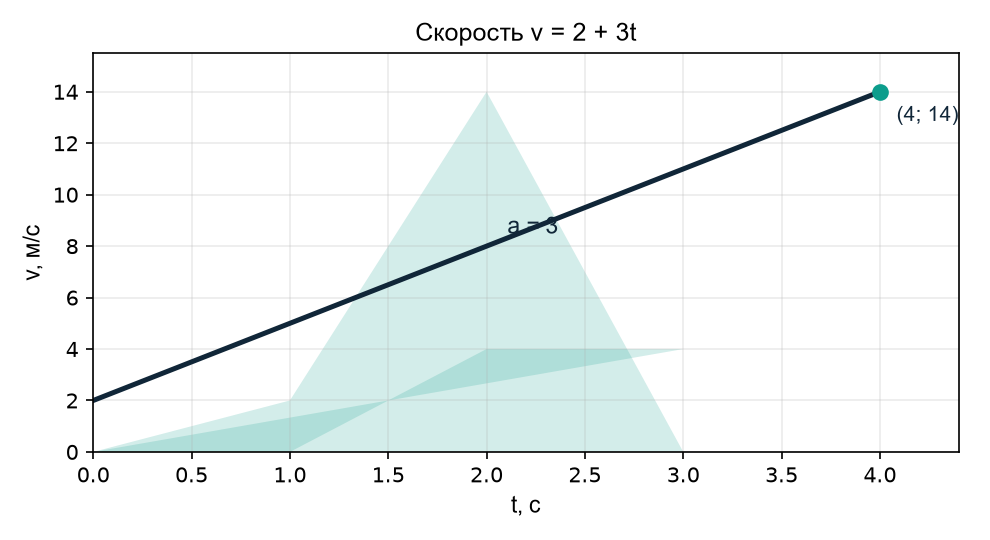
\includegraphics[width=0.85\textwidth]{fig_vt_ru.png}
\caption{График скорости v = 2 + 3t. Наклон прямой равен ускорению a = 3 м/с$^2$; закрашенная площадь под графиком численно равна перемещению s = 32 м.}
\end{figure}
\begin{figure}[h]
\centering
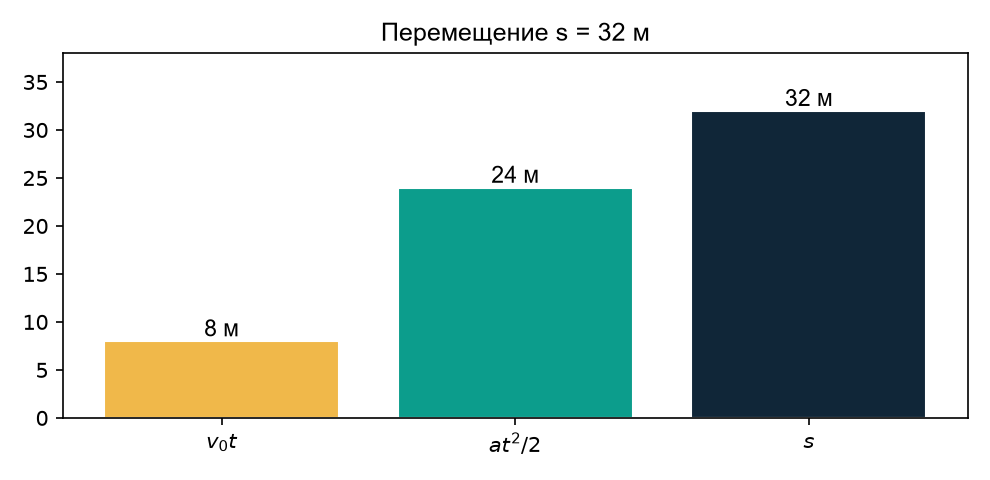
\includegraphics[width=0.85\textwidth]{fig_bars_ru.png}
\caption{Слагаемые перемещения: v$_0$t = 8 м (без разгона) и at$^2$/2 = 24 м (добавка от разгона); итого s = 32 м.}
\end{figure}
\section*{Решённый пример}
Условие: v$_0$ = 2 м/с, a = 3 м/с$^2$, t = 4 с. Найти v и s.
\begin{enumerate}
\item Скорость: v = v$_0$ + at = 2 + 3$\cdot$4 = 14 м/с.
\item Перемещение: s = v$_0$t + at$^2$/2 = 2$\cdot$4 + 3$\cdot$16/2 = 8 + 24 = 32 м.
\item Проверка площадью: s = (v$_0$ + v)t/2 = (2 + 14)$\cdot$4/2 = 32 м. Сошлось.
\end{enumerate}
Пауза-задача (B6): v$_0$ = 0, a = 2 м/с$^2$, t = 5 с $\to$ s = 0$\cdot$5 + 2$\cdot$25/2 = 25 м.
\section*{Задания для самостоятельной работы}
Реши сам; ответы — в отдельном разделе.


\textbf{H1.} Тело движется с начальной скоростью 2 м/с и ускорением 3 м/с$^2$. Найдите скорость через 4 секунды.

\textbf{A.} 14 м/с \\
\textbf{B.} 12 м/с \\
\textbf{C.} 9 м/с \\
\textbf{D.} 6 м/с

\textbf{H2.} Тело движется с начальной скоростью 2 м/с и ускорением 3 м/с$^2$. Найдите перемещение за 4 с. Направление движения не меняется.

\textbf{A.} 32 м \\
\textbf{B.} 56 м \\
\textbf{C.} 24 м \\
\textbf{D.} 20 м

\textbf{H3.} Какое движение называется равноускоренным?

\textbf{A.} Скорость за равные промежутки времени меняется одинаково \\
\textbf{B.} Скорость постоянна \\
\textbf{C.} Ускорение меняется со временем \\
\textbf{D.} Путь за равные промежутки времени одинаков

\textbf{H4.} Что показывает наклон прямой на графике скорости от времени?

\textbf{A.} Ускорение \\
\textbf{B.} Перемещение \\
\textbf{C.} Скорость \\
\textbf{D.} Время

\textbf{H5.} На графике v(t) прямая идёт от точки (0 с; 2 м/с) до точки (4 с; 14 м/с). Найдите перемещение.

\textbf{A.} 32 м \\
\textbf{B.} 48 м \\
\textbf{C.} 56 м \\
\textbf{D.} 24 м
\clearpage
\section*{Ответы}
Ответы и короткие пояснения.
\textbf{H1 — A} (14 м/с). Ускорение каждую секунду увеличивает скорость на 3 м/с. Поэтому v = v$_0$ + at = 2 + 3$\cdot$4 = 14 м/с.
\textbf{H2 — A} (32 м). s = v$_0$t + at$^2$/2 = 2$\cdot$4 + 3$\cdot$16/2 = 8 + 24 = 32 м. Вариант 56 м получается, если подставить конечную скорость в формулу равномерного движения.
\textbf{H3 — A} (Скорость за равные промежутки времени меняется одинаково). Равноускоренное движение — скорость получает равные прибавки за равные времена при постоянном ускорении (Закирова 9, §3). Вариант D описывает равномерное движение.
\textbf{H4 — A} (Ускорение). Наклон v(t) равен ускорению: a = $\Delta$v/$\Delta$t. Перемещение — это площадь под графиком, а не наклон (Закирова 10, §3).
\textbf{H5 — A} (32 м). Площадь трапеции: (2 + 14)/2 $\cdot$ 4 = 32 м. Вариант 24 м — только треугольник без прямоугольника.
\section*{Источники}
\begin{itemize}
\item Закирова, Физика, 9 кл., §3 — равноускоренное движение, графики v(t) (PDF с. 19–26).
\item Закирова, Физика, 10 кл. ЖМ, §3 — уравнения кинематики, наклон и площадь графика v(t) (PDF с. 15–18, 20).
\item Закирова, Физика, 11 кл. ЖМ — перекрёстная проверка обозначений (PDF с. 8–12).
\item «369 формула» — перекрёстная проверка формул (PDF с. 6–7).
\item FBS — перекрёстная проверка обозначений и единиц (PDF с. 6–7).
\item Сборники ЕНТ: \url{https://testcenter.kz}
\end{itemize}
Источники использованы только для сверки; тексты, рисунки и задания учебников не воспроизводятся.
\end{document}
